% !TeX spellcheck = cs_CZ
%{\tikzset{external/prefix={tikz/FYZII/}}
% \tikzset{external/figure name/.add={ch06_}{}}
%---------------------------------------------------------------------------------------------------
% file fey1ch08.tex
%---------------------------------------------------------------------------------------------------
%====================Kapitola: Elektrostatická energie =============================================
\setchaptertoc
\chapter{Elektrostatická energie}\label{fyz:IIchapVI}
  \section{Elektrostatická energie nábojů. Homogenní koule}\label{fyz:IIchapVIsecI}
    Jedním z nejzajímavějších a nejužitečnějších objevů v mechanice byl zákon zachování energie.
    Vzorce pro kinetickou a potenciální energii mechanické soustavy nám pomáhají objevit souvislosti
    mezi stavy soustavy ve dvou různých časech, aniž bychom museli vnikat do podrobností toho, co se
    mezi tím děje. Nyní se chceme zabývat energií elektrostatických soustav. I v nauce o elektřině
    bude princip zachování energie užitečný při objevování mnoha zajímavých věcí.

    Zákon o energii vzájemného působení je v elektrostatice velmi jednoduchý; vlastně jsme ho již
    probírali. Představte si, že máme dva náboje \(q_1\) a \(q_2\) vzdálené od sebe o \(r_{12}\).
    Tato soustava se vyznačuje nějakou energií, neboť na to, aby se oba náboje přivedly do jejich
    současné vzájemné polohy, bylo třeba vynaložit určité množství práce. Práci, která je vykonána
    při přiblížení dvou nábojů z velké vzdálenosti, jsme už počítali. Je rovna
    \begin{equation}\label{fyz:eq868}
      \dfrac{q_1q_2}{4π\varepsilon_0r_{12}}.      
    \end{equation}
    Kromě toho z principu superpozice víme, že v případě mnoha nábojů je celková síla působící na
    každý z nich rovna součtu sil, kterými na něj působí všechny ostatní náboje. Z toho vyplývá, že
    celková energie soustavy více nábojů je rovna součtu členů pocházejících ze vzájemné interakce
    každého páru nábojů. Jsou-li \(q_i\) a \(q_j\) některé dva z těchto nábojů a \(r_{12}\) je
    vzdálenost mezi nimi (\ref{fyz:fig0178}), energie tohoto páruje
    \begin{equation}\label{fyz:eq869}
      \dfrac{q_iq_j}{4π\varepsilon_0r_{ij}}.      
    \end{equation}

    \begin{figure}[ht!]  %\ref{fyz:fig0178}
      \centering
      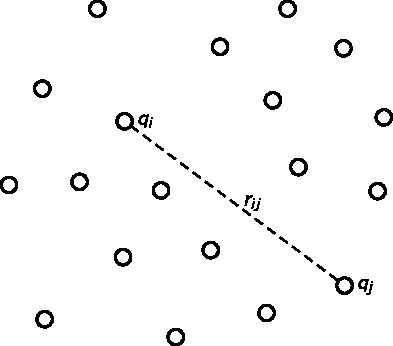
\includegraphics[width=0.6\linewidth]{fyz_fig0178.pdf}
      \caption{Elektrostatická energie soustavy částic je rovna součtu elektrostatických energií
              všech párů částic v soustavě (\cite[s.~140]{Feynman02}).}
      \label{fyz:fig0178}
    \end{figure}

    Výsledná elektrostatická energie \(W\) je součtem energií všech možných párů nábojů v soustavě:
    \begin{equation}\label{fyz:eq870}
      W=\sum_{\mathclap{\substack{\text{všechny}\\\text{páry}}}}\dfrac{q_iq_j4π\varepsilon_0}{r_{ij}}.
    \end{equation}
    Jde-li o rozdělení nábojů specifikované hustotou náboje \(ρ\), je samozřejmě nutné nahradit sumu
    ve vzorci (\ref{fyz:eq870}) integrálem.

    My se budeme touto energií zabývat ze dvou hledisek. Jedním je \emph{využití} pojmu energie v
    elektrostatických úlohách a druhým jsou různé způsoby výpočtu energie. Někdy je snazší vypočítat
    práci vykonanou v nějakém speciálním případě, než vyčíslit sumu nebo příslušný integrál ve
    vzorci (\ref{fyz:eq870}). Jako příklad vypočtěme energii potřebnou na shromáždění náboje do
    koule s homogenní hustotou náboje. Je rovna práci vykonané při přibližování nábojů z nekonečna.

    Představte si, že kouli vytváříme postupným přikládáním tenkých kulových slupek s
    infinitezimální tloušťkou na sebe. V každém stádiu tohoto procesu bereme malé množství náboje a
    přikládáme jej ve tvaru tenké kulové slupky sahající od \(r\) do \(r + \dd{r}\).

    \begin{figure}[ht!]  %\ref{fyz:fig0179}
      \centering
      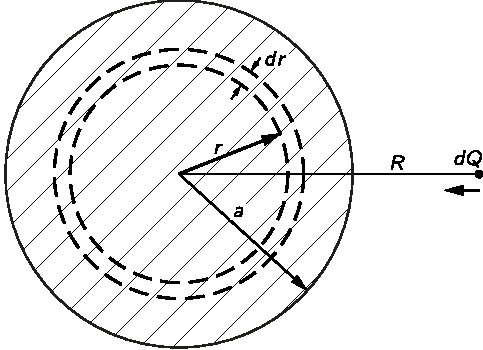
\includegraphics[width=0.6\linewidth]{fyz_fig0179.pdf}
      \caption{Energii homogenně nabité koule můžeme počítat tak, že si představíme kouli, jako by
              byla složena ze vzájemně na sebe přiléhajících kulových slupek.
              (\cite[s.~141]{Feynman02}).}
      \label{fyz:fig0179}
    \end{figure}

    Pokračujeme tak dlouho, dokud nedosáhneme konečného poloměru a (obr. \ref{fyz:fig0179}). Je-li
    náboj koule ve stádiu, kdy byla vytvořena do poloměru \(r\), je při přinášení dalšího náboje
    \(\dd{Q}\) vykonávána práce.
    \begin{equation}\label{fyz:eq871}
      \dd{W}=\dfrac{Q}{r^4π\varepsilon_0r}\dd{Q}.
    \end{equation}
    Je-li hustota náboje v kouli \(ρ\), náboj \(Q_r\) je
    \begin{equation*}
      Q_r=ρ\cdot\dfrac{4}{3}πr^3,
    \end{equation*}
    a náboj \(\dd{Q}\) je vyjádřen takto:
    \begin{equation*}
      \dd{Q}=ρ⋅4πr^2\dd{r}.
    \end{equation*}
    Rovnost (\ref{fyz:eq871}) pak získá tvar
    \begin{equation}\label{fyz:eq872}
      \dd{W}=\dfrac{4πρ^2r^4\dd{r}}{3\varepsilon_0}.
    \end{equation}
    Celková energie potřebná na vytvoření koule je rovna integrálu \(\dd{W}\) od \(r = 0\) do \(r =
    a\), tj.
    \begin{equation}\label{fyz:eq873}
      W=\dfrac{4πρ^2a^5}{15\varepsilon_0}.
    \end{equation}
    Chceme-li výsledek vyjádřit pomocí celkového náboje \(Q\) koule, dostaneme
    \begin{equation}\label{fyz:eq874}
      W=\dfrac{3}{5}\dfrac{Q^2}{4π\varepsilon_0a}.
    \end{equation}
    Energie je tedy přímo úměrná druhé mocnině celkového náboje a nepřímo úměrná poloměru. Vztah
    (\ref{fyz:eq874}) můžeme interpretovat také tak, že podle něj je střední hodnota veličiny
    (\(1/r_{ij}\)) pro všechny páry bodů v kouli \(3/5 a\).

  \twocolumn[\section{Energie kondenzátoru. Síly působící na nabité vodiče}\label{fyz:IIchapVIsecII}]
    Nyní uvažujme o energii potřebné k nabití kondenzátoru. Vezmeme-li od jednoho z vodičů tvořících
    kondenzátor náboj \(Q\) a přeneseme-li ho na druhý vodič, vznikne mezi nimi rozdíl potenciálů
    \begin{equation}\label{fyz:eq875}
      U = \dfrac{Q}{C},
    \end{equation}
    kde \(C\) je kapacita kondenzátoru. Kolik práce je vykonáno při nabíjení kondenzátoru? Budeme
    postupovat stejně jako v případě koule a představíme si, že kondenzátor se nabíjel přenášením
    náboje po malých částech \(\dd{Q}\), z jedné jeho desky na druhou. Na přenesení náboje
    \(\dd{Q}\) je spotřebována práce
    \begin{equation*}
      \dd{W} = U\dd{Q}.
    \end{equation*}
    Dosazením \(U\) z (\ref{fyz:eq875}) tento vztah získá tvar
    \begin{equation*}
      \dd{U} = \dfrac{Q\dd{Q}}{C}.
    \end{equation*}
    Když potom integrujeme od nulového do konečného náboje \(Q\) dostaneme
    \begin{align}
      W &= \dfrac{1}{2}\dfrac{Q^2}{C}.  \label{fyz:eq876}     \\
      \shortintertext{Tuto energii je možné napsat i ve tvaru}
      W &= \dfrac{1}{2}CU^2.            \label{fyz:eq877}
    \end{align} 

    Vzpomeneme-li si, že kapacita vodivé koule (vzhledem k nekonečnu) je
    \begin{equation*}
      C_{\text{koule}} = 4π\varepsilon0a,
    \end{equation*}
    můžeme ze vzorce (\ref{fyz:eq876}) ihned dostat vztah pro energii nabité koule:
    \begin{equation}\label{fyz:eq878}
      W=\dfrac{1}{2}\dfrac{Q^2}{4π\varepsilon_0a}.
    \end{equation}
    Ovšem toto je i vztah pro energii \emph{tenké kulové slupky} s celkovým nábojem \(Q\) tato
    energie představuje \(5/6\) energie homogenně nabité koule, vyjádřené vztahem (\ref{fyz:eq874}).

    Nyní se zabývejme aplikacemi pojmu elektrostatické energie. Zkoumejme následující otázky: Jaká
    síla působí mezi elektrodami kondenzátoru? Nebo: Jaký moment síly vzhledem k nějaké ose působí
    na nabitý vodič v přítomnosti jiného vodiče s opačným nábojem? Takové otázky lze snadno
    zodpovědět použitím našeho výsledku (\ref{fyz:eq877}) pro elektrostatickou energii kondenzátoru
    spolu s principem virtuální práce (viz kapitoly \ref{fyz:IchapIV}, a \ref{fyz:IchapXIII},
    díl \ref{part:FYZI}).

    Použijeme tuto metodu na určení síly působící mezi deskami rovinného kondenzátoru.
    Představíme-li si, že mezera mezi deskami se zvětšila o malou hodnotu \(\Delta z\), mechanická
    práce vynaložená vnější silou na posunutí desek byla
    \begin{equation}\label{fyz:eq879}
      ΔA=FΔz,
    \end{equation}
    kde \(F\) je síla působící mezi deskami. Tato práce musí být rovna změně elektrostatické energie
    kondenzátoru.

    Podle vztahu (\ref{fyz:eq876}) měl kondenzátor původně energii
    \begin{equation*}
      W = \dfrac{1}{2}\dfrac{Q^2}{C}.
    \end{equation*}
    Změna energie (nedopustíme-li, aby se náboj změnil) je
    \begin{equation}\label{fyz:eq880}
      ΔW=\dfrac{1}{2}Q^2Δ\left(\dfrac{1}{C}\right).
    \end{equation}
    Porovnáním (\ref{fyz:eq879}) a ({fyz:eq880}) dostaneme
    \begin{align}
      FΔz &=\dfrac{Q^2}{2}Δ\left(\dfrac{1}{C}\right). \label{fyz:eq881} \\
      \shortintertext{což je možné napsat ve tvaru}
      FΔz &=−\dfrac{Q^2}{2C^2}ΔC.                     \label{fyz:eq882}
    \end{align}
    Působící síla, samozřejmě, vyplývá z rozdělení nábojů na deskách, ale jak je vidět, nemusíme se
    starat o jejich detailní rozdělení; všechno, co potřebujeme, je obsaženo v kapacitě \(C\)

    \begin{figure}[ht!]  %\ref{fyz:fig0180}
      \centering
      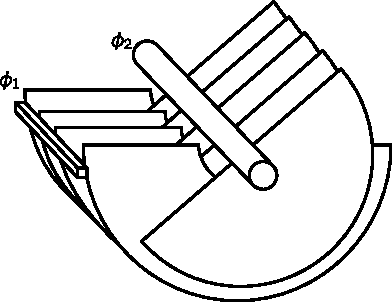
\includegraphics[width=0.6\linewidth]{fyz_fig0180.pdf}
      \caption{Jaký moment síly působí na otočný kondenzátor? (\cite[s.~144]{Feynman02}).}
      \label{fyz:fig0180}
    \end{figure}

    Je zřejmé, že tuto myšlenku lze rozšířit na vodiče jakéhokoliv tvaru a na ostatní složky síly.
    Ve vztahu (\ref{fyz:eq881}) zaměníme \(F\) složkou, kterou hledáme, a \(\Delta z\) nahradíme
    malým posunutím v odpovídajícím směru. Nebo máme-li elektrodu vyznačující se nějakou osou a je
    třeba najít moment síly \(τ\), napíšeme virtuální práci ve tvaru
    \begin{equation*}
      ΔA=τΔθ,
    \end{equation*}
    kde \(Δθ\) je malé \emph{úhlové posunutí}. V tomto případě musí \(Δ(1/C)\) přirozeně
    představovat změnu veličiny \(1/C\) příslušnou pootočení \(Δθ\). Tak bychom mohli najít moment
    působící na pohyblivé desky v otočném kondenzátoru takového typu, jako je na obr.
    \ref{fyz:fig0181}.
    
    Vrátíme se ke speciálnímu případu kondenzátoru s rovnoběžnými rovinnými elektrodami. Pro jeho
    kapacitu můžeme použít vzorec odvozený v kapitole \ref{fyz:IIchapV}:
    \begin{equation}\label{fyz:eq883}
      \dfrac{1}{C}=\dfrac{d}{\varepsilon_0S},
    \end{equation}
    kde \(S\) je plošný obsah každé desky. Zvětšíme-li mezeru mezi deskami o \(\Delta z\), bude
    platit
    \begin{equation*}
      Δ\left(1C\right)=\dfrac{Δz}{\varepsilon_0S}.
    \end{equation*}
    Z rovnice (\ref{fyz:eq881}) dostaneme, že síla mezi deskami je
    \begin{equation}\label{fyz:eq884}
      F=\dfrac{Q^2}{2\varepsilon_0S}.
    \end{equation}
    Všimněme si výrazu (\ref{fyz:eq881}) trochu blíže a podívejme se, zda lze říci, jak tato síla
    vzniká. Vyjádříme-li náboj na jedná desce ve tvaru
    \begin{equation*}
      Q=σS,
    \end{equation*}
    vztah (\ref{fyz:eq884}) lze přepsat takto:
    \begin{equation*}
      F=\dfrac{1}{2}Q\dfrac{σ}{\varepsilon_0}.
    \end{equation*}
    Protože intenzita elektrického pole mezi deskami je
    \begin{equation*}
      E_0=\dfrac{σ}{\varepsilon_0},
    \end{equation*}
    máme
    \begin{equation}\label{fyz:eq885}
      F=\dfrac{1}{2}QE_0.
    \end{equation}

    Ihned bylo možné se dovtípit, že síla působící na jednu desku je rovna součinu náboje \(Q\) na
    desce a intenzity pole působícího na náboj. Dostali jsme však překvapující součinitel \(1/2\).
    Příčina spočívá v tom, že \(E_0\) není ta intenzita pole, která je v místě, kde jsou náboje.
    Když si představíme, že náboj zabírá tenkou vrstvu na povrchu desky, jak to znázorňuje obr.
    \ref{fyz:fig0181}, intenzita pole se bude měnit od nuly na vnitřním okraji vrstvy do \(E_0\) v
    prostoru mimo desku.
    
    \begin{figure}[ht!]  %\ref{fyz:fig0181}
      \centering
      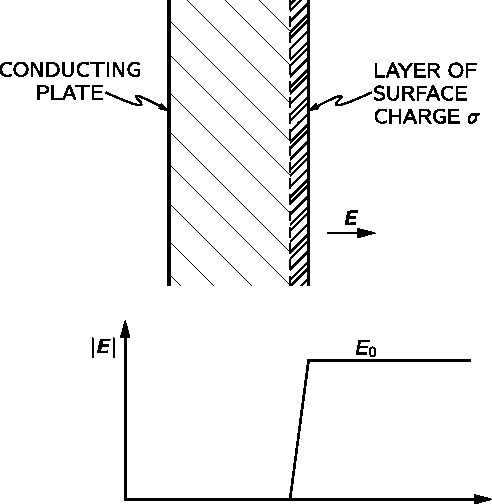
\includegraphics[width=0.8\linewidth]{fyz_fig0181.pdf}
      \caption{Intenzita elektrického pole se změní při průchodu vrstvou plošného náboje
              existujícího na povrchu vodiče z nuly na hodnotu \(E_0 =
              \frac{\sigma}{\varepsilon_0}\) (\cite[s.~145]{Feynman02}).}
      \label{fyz:fig0181}
    \end{figure}

    Střední intenzita působící na náboje je \(E_0/2\). To je důvod, proč ve vztahu (\ref{fyz:eq885})
    vystupuje součinitel \(1/2\).

    Je nutné, abychom si všimli, že při výpočtu virtuální práce jsme předpokládali, že náboj na
    kondenzátoru je stálý, tj. že kondenzátor není elektricky připojen k jiným tělesům, a tak se
    celkový náboj nemůže měnit. 
    
    Předpokládejme, že po dobu virtuálního přemístění by se kondenzátor udržoval na stálém rozdílu
    potenciálů. V tom případě bychom měli použít vztah
    \begin{equation*}
      W = \dfrac{1}{2}CU^2.
    \end{equation*}
    a místo (\ref{fyz:eq882}) bychom dostali
    \begin{equation*}
      FΔz=\dfrac{1}{2}U^2ΔC,
    \end{equation*}
    z čehož vyplývá stejně velká síla jako ze vztahu (\ref{fyz:eq882}) (neboť \(U= Q/C\)), ale s
    opačným znaménkem. Tím, že jsme kondenzátor odpojili od nabíjecího zdroje, síla mezi jeho
    elektrodami zajisté nezmění znaménko. Kromě toho víme, že dvě elektrody s opačnými elektrickými
    náboji se musí přitahovat. V druhém případě však byl princip virtuální práce použit nekorektně -
    nevzali jsme v úvahu virtuální práci vykonanou nabíjecím zdrojem. Aby se totiž při změně
    kapacity udržel stejný potenciál \(U\), je nutné, aby zdroj dodal náboj \(U\Delta C\). Tento
    náboj je však dodáván při potenciálu \(U\), takže práce konaná elektrickým systémem udržujícím
    neměnný potenciál, je \(U^2\Delta C\). Mechanická práce \(F\Delta z\) \emph{plus} elektrická
    práce \(U^2\Delta C\) spolu dávají změnu celkové energie kondenzátoru rovnou —
    \(\frac{1}{}U^2\Delta C\). Proto \(FΔz=−\frac{1}{2}V^2ΔC\) stejně jako předtím.
    
  \twocolumn[\section{Elektrostatická energie iontového krystalu}\label{fyz:IIchapVIsecIII}] 
  
    Nyní se zabývejme využitím pojmu elektrostatické energie v atomové fyzice. Síly mezi atomy nelze
    méřit snadno, ale často nás zajímají rozdíly energie mezi dvěma konfiguracemi atomů, např.
    energie chemických změn. Protože atomové síly jsou v podstatě elektrickými silami, chemické
    energie jsou z velké části právě elektrostatickými energiemi.
    
    Uvažujme například elektrostatickou energii iontové mřížky. Iontový krystal, tj. takový jako je
    krystal \ce{NaCl}, se skládá z kladných a záporných iontů, které je možné považovat za tuhé
    koule. Elektricky se přitahují, dokud se nezačnou vzájemně dotýkat; potom se uplatní odpudivá
    síla, která velmi prudce vzroste, pokusíme-li s eje přiblížit těsněji.
    
    Proto jako naše první přiblížení vezměme soustavu tuhých koulí, představující atomy v krystalu
    kuchyňské soli. Struktura krystalové mřížky byla určena pomocí ohybu rentgenového záření. Jde o
    kubickou mřížku (jako trojrozměrná šachovnice). Obr. \ref{fyz:fig0182} ukazuje její řez.
    Vzdálenost mezi sousedními ion tyje \SI{0.281}{\nm} (=\SI{2.81e-10}{\m}).
    
    \begin{figure}[ht!]  %\ref{fyz:fig0182}
      \centering
      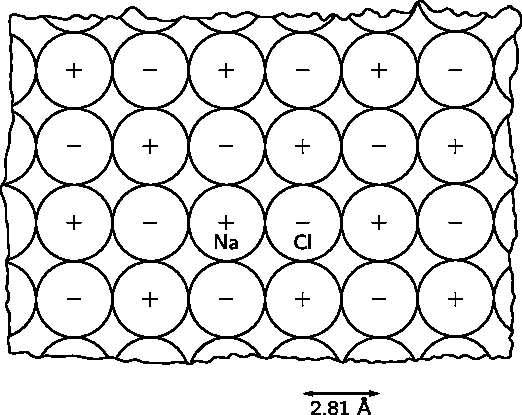
\includegraphics[width=0.6\linewidth]{fyz_fig0182.pdf}
      \caption{Řez krystalem kuchyňské soli v atomovém měřítku. Šachovnicové uspořádání iontů \ce{Na} 
              a \ce{Cl} je stené v obou na sebe kolmých řezech krystalem (obr. \ref{fyz:fig0013} díl
              \ref{part:FYZI}) (\cite[s.~146]{Feynman02}).}
      \label{fyz:fig0182}
    \end{figure}

    Je-li náš obraz této soustavy správný, měli bychom být schopni provéřit jej tím, že si položíme
    následující otázku: Kolik energie je třeba, aby se všechny tyto ionty od sebe navzájem oddělily,
    tj. aby se krystal úplně rozbil na jednotlivé ionty? Tato energie bude rovna skupenskému teplu
    vypařování \ce{NaCl} zvětšená o energii potřebnou na disociaci molekul na ionty. Celková energie
    potřebná na rozdrobení \ce{NaCl} na ionty byla experimentálně určena jako \num{7.92}
    elektronvoltů na jednu molekulu. Použijeme-li převod
    \begin{equation*}
      \SI{1}{\electronvolt} = \SI{1.602e-19}{\joule}
    \end{equation*}
    a Avogadrovu konstantu jako počet molekul v jednom molu, tedy
    \begin{align*}
      N_0 &= \SI{6.02e23}{\per\mole},  \\
      \shortintertext{energii vypařování napíšeme takto:}
      W   &= \SI{7.64}{\joule\per\mole}.
    \end{align*}

    Je možné dostat tuto chemickou energii teoreticky vypočítáním množství práce potřebné k
    roztržení krystalu? Podle naší teorie představuje tato práce součet potenciálních energií všech
    iontových párů. Nejsnadnější cestou pro výpočet tohoto součtu je vybrat vždy konkrétní ion a
    počítat jeho potenciální energii vzhledem ke každému z ostatních iontů. Dostaneme tak
    \emph{dvojnásobek} energie připadající najeden ion, protože počítané energie budou náležet párům
    iontů. Potřebujeme-li, aby se vypočítaná energie vztahovala k jedinému konkrétnímu iontu, musíme
    vzít poloviční hodnotu. Ale ve skutečnosti potřebujeme energii připadající na \emph{jednu
    molekulu}, která obsahuje dva ionty, takže vypočtený součet bude přímo udávat energii
    připadající na molekulu.

    Energie iontu vzhledem k jednomu z jeho nebližších sousedů je rovna \(e^2/a\), kde
    \(e^2=q^2e/4π\varepsilon_0\) a \(a\) je vzdálenost mezi středy obou iontů. (Uvažujeme jednovazné
    ionty.) Tato energie je rovna \SI{5.12}{\electronvolt}, což, jak už vidíme, by nám mělo
    poskytnout výsledek o řádově správné velikosti. Ale do nekonečné sumy, kterou potřebujeme
    spočítat, je ještě dlouhá cesta.

    Začněme sčítáním všech členů, které pocházejí od iontů ležících v jedné přímce.
    Předpokládáme-li, že ion označený \ce{Na} na obr. \ref{fyz:fig0182} je naším konkrétním iontem,
    uvažme nejdříve ty ionty, které s ním leží na jedné vodorovné přímce. Nejbližší jsou dva záporně
    nabité ionty \ce{Cl}, každý ve vzdálenosti \(a\). Potom jsou dva kladné ionty ve vzdálenosti
    \(2a\) atd. Označíme-li energii, kterou dá tento součet \(W_1\), bude platit
    \begin{align*}
      W &= \dfrac{e^2}{a}\left(−\dfrac{2}{1}+\dfrac{2}{2}−\dfrac{2}{3}+\dfrac{2}{4}∓\cdots\right) \\
        &=−\dfrac{2e^2}{a}\left(1−\dfrac{1}{2}+\dfrac{1}{3}−\dfrac{1}{4}±\cdots\right).
    \end{align*}
    Tato řada konverguje pomalu, takže je těžké ji numericky vyčíslit. Je však známo, že je rovna
    \(\ln2\). Tedy
    \begin{equation}\label{fyz:eq886}
      W_1=−\dfrac{2e^2}{a}\ln2=−\num{1.386}\dfrac{e^2}{a}.
    \end{equation}

    Nyní uvažujme přímku iontů, která sousedí s už uvažovanou přímkou shora. Nejbližší iont je
    záporný a je ve vzdálenosti \(a\). Potom jsou dva kladné ionty ve vzdálenosti \(\sqrt{2}a\),
    další ve vzdálenosti \(\sqrt{5}a\) a další \(\sqrt{10}a\) atd. Takto pro celou přímku dostáváme
    řadu
    \begin{equation}\label{fyz:eq887}
      \dfrac{e^2}{a}\left(−\dfrac{1}{1}+\dfrac{2}{\sqrt{2}}
                          –\dfrac{2}{\sqrt{5}}+\dfrac{2}{\sqrt{10}}∓\cdots
                    \right).
    \end{equation}

    Takové přímky existují čtyři: shora, zdola, zepředu a zezadu. Potom jsou čtyři přímky, jež jsou
    nejbližšími přímkami na úhlopříčkách atd., atd.

    Zpracujete-li trpělivě všechny přímky a pak uděláme sumu, dostanete konečný výsledek
    \begin{equation*}
      W=−\num{1.747}e^2a,
    \end{equation*}
    což je pouze o něco víc, než jsme dostali v (8.20) pro první přímku. Dosadíme-li \(e^2/a =
    \SI{5.12}{\electronvolt}\), 
    \begin{equation*}
      W=−\SI{8.94}{\electronvolt}.
    \end{equation*}

    Náš výsledek převyšuje asi o \SI{10}{\percent} experimentálně pozorovanou energii. To ukazuje,
    že naše představa o mřížce jako útvaru drženém pohromadě elektrickými Coulombovými silami, je v
    podstatě správná. Je to poprvé, kdy jsme dostali specifickou vlastnost makroskopické látky na
    základě po­znání atomové fyziky. Později dosáhneme mnohem víc. Předmět, jenž se snaží vysvětlit
    vlastnosti makroskopických množství látky pomocí zákonů chování atomů, se nazývá \emph{fyzika
    pevných látek}.

    A jak je to s chybou našeho výpočtu? Proč tento výpočet neplatí přesně? Pro odpuzování mezi
    ionty na krátké vzdálenosti. Nejsou to dokonale tuhé koule, takže když jsou těsně u sebe,
    částečně se stlačí. Jelikož nejsou příliš měkké, stlačí se jen trochu. Na jejich deformaci je
    však spotřebována nějaká energie a když se ionty od sebe vzdalují, tato energie se uvolňuje.
    Skutečná energie potřebná k oddělení iontů je trochu menší než ta, kterou jsme vypočítali;
    jejich vzájemné odpuzování pomáhá překonat elektrostatické přitahování.

    Existuje nějaký způsob, jak můžeme určit tento příspěvek? Mohli bychom, kdybychom znali zákon
    odpudivé síly. Nejsme připraveni na analýzu detailů tohoto mechanismu odpuzování. Určitou
    představu o jeho charakteristikách však můžeme získat z některých makroskopických měření. Z
    měření stlačitelnosti celého krystalu můžeme získat kvantitativní představu o zákonu odpuzování
    mezi ionty, a tím o jeho příspěvku k energii. Takovou cestou bylo zjištěno, že tento příspěvek
    musí být 1/9,4 příspěvku elektrického přitahování a má, samozřejmě, opačné znaménko. Odečteme-li
    tento příspěvek od čisté elektrostatické energie, dostaneme \SI{7.99}{\electronvolt} jako
    energii disociace připadající na jednu molekulu. Je to mnohem blíže k pozorované hodnotě
    \SI{7.92}{\electronvolt}, ale stále ještě ne dokonale shodné. Existuje ještě jedna věc, kterou
    jsme nevzali v úvahu - vůbec jsme nezapočítali kinetickou energii kmitů mřížky. Když se udělá
    oprava i na tento efekt, získá se velmi dobrá shoda s experimentální hodnotou. Naše představy
    jsou pak správné; hlavním příspěvkem k energii takového krystalu, jako je \ce{NaCl}, je
    elektrostatická energie.

  \twocolumn[\section{Elektrostatická energie v atomových jádrech}\label{fyz:IIchapVIsecIV}]
    Nyní se budeme věnovat jinému příkladu elektrostatické energie v atomové fyzice - elektrické
    energii atomových jader. Předtím však musíme pohovořit o některých vlastnostech hlavních sil
    (nazvaných jaderné síly), které udržují protony a neutrony v jádře pohromadě. V prvním období po
    objevu jader, jakož i neutronů a protonů, jež je vytvářejí, fyzici doufali, že silná
    neelektrická část síly působící mezi, řekněme, protonem a jiným protonem bude vyjádřena nějakým
    jednoduchým zákonem, podobným zákonu nepřímé úměrnosti druhé mocnině vzdálenosti v případě
    elektřiny. Kdyby byl tento zákon jednou určen, jakož i odpovídající zákony sil působících mezi
    protonem a neutronem a mezi neutronem a neutronem, bylo by možné teoreticky popsat celé chování
    těchto částic v jádrech. Proto byl zahájen rozsáhlý program výzkumu rozptylu protonů v naději,
    že bude nalezen zákon síly působící mezi nimi; ale ani po třiceti letech úsilí nevyšlo najevo
    nic jednoduchého. O síle, která působí mezi protonem a protonem byl nashromážděno velké množství
    poznatků, ale zjišťujeme, že jde o tak složitou sílu, jak jen může být.

    \begin{figure}[ht!]  %\ref{fyz:fig0183}
      \centering
      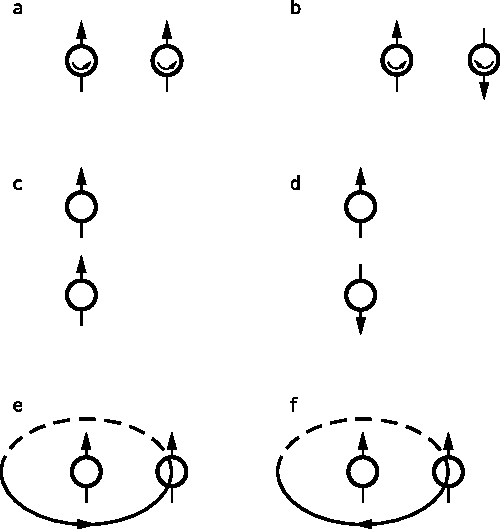
\includegraphics[width=0.8\linewidth]{fyz_fig0183.pdf}
      \caption{Síla mezi dvěma protony závisí na všech možných parametrech.
              (\cite[s.~148]{Feynman02}).}
      \label{fyz:fig0183}
    \end{figure}

    Výrokem „tak složitá, jak jen může být“ myslíme, že tato síla závisí na takovém množství
    činitelů, jak je to jen možné.
    
    Zaprvé, síla není jednoduchou funkcí vzdálenosti mezi oběma protony. Při velkých vzdálenostech
    jde o přitahování, ale při těsnějších vzdálenostech nastává odpuzování. Závislost na vzdálenosti
    představuje složitou, stále ještě ne zcela známou funkci. Za druhé, síla závisí na orientaci
    spinů protonů. Protony mají spin (představujeme si jej prostě jako rotaci kolem své vlastní osy)
    a každé dva interagující protony mohou rotovat s momenty hybnosti ve stejném směru nebo ve
    směrech opačných. A síla, když jsou spiny paralelní, je různá od síly, když jsou antiparalelní.
    (obr.\ref{fyz:fig0183} a, b). Rozdíl je velmi velký, a nejde tedy o malý efekt.

    Za třetí, síla v případě, že spojnice mezi oběma protony leží ve směru rovnoběžném jejich spiny
    (obr. \ref{fyz:fig0183} c, d) se značně liší od síly v případě, kdy má spojnice směr kolmý na
    spiny, jako na obr. \ref{fyz:fig0183} a, b.

    Za čtvrté, síla - podobné jako je tomu v magnetismu - závisí na rychlosti protonů, ale mnohem
    silněji než v magnetismu. Tato síla, závisící na rychlosti, není relativistickým efektem; velká
    je i při rychlostech mnohem menších než rychlost světla. Kromě toho tato část síly závisí i na
    jiných faktorech než na velikosti rychlosti. Například pohybuje-li se proton blízko jiného
    protonu, liší se síla podle toho, zda orbitální pohyb má stejný (obr. \ref{fyz:fig0183} e) nebo
    opačný (obr. \ref{fyz:fig0183} f) směr rotace jako spin. S tímto souvisící část síly je nazývána
    \emph{spin-orbitální část} jaderné síly.

    Síly mezi protonem a neutronem nebo mezi neutronem a neutronem jsou stejně komplikované. Do
    dnešního dne neznáme mechanismus těchto sil, tj. nějaký jednoduchý způsob, jak je pochopit.

    V jednom ohledu jsou však síly mezi nukleony jednodušší, než by mohly být. Jde o to, že jaderná
    síla mezi dvěma neutrony je stejná jako mezi protonem a neutronem a tatáž jako síla mezi dvěma
    protony. Nahradíme-li v jakékoliv jaderné konfiguraci proton neutronem (nebo naopak), jaderné
    interakce se nezmění. „Základní příčina“ této rovnosti je známa, ale jde o příklad důležitějšího
    principu, který je možné rozšířit i na zákony interakce jiných částic vyznačující se silnými
    interakcemi, např. pionů a „podivných“ částic.

    Tento fakt lze pěkně ilustrovat rozmístěním hladin energie v podobných jádrech. Uvažujme takové
    jádro jako \ce{^11B} (bór jedenáct), jež se skládá z pěti protonů a šesti neutronů. Těchto
    jedenáct částic v jádře na sebe navzájem působí nejsložitějším způsobem. Existuje jedna
    konfigurace ze všech možných interakcí, jež má nejnižší možnou energii - je to normální stav
    jádra a nazývá se základní stav. Vybudí-li se jádro (například nárazem protonu nebo jiné částice
    s vysokou energií), je možné přivést jej do nekonečně mnoha jiných konfigurací, nazvaných
    excitované stavy, z nichž každý bude mít charakteristickou energii větší, než je energie
    základního stavu. Ve výzkumech fyziky jádra, např. takových, jako se dělají pomocí van de
    Graaffova generátoru, se experimentálně určují energie a další vlastnosti těchto vybuzených
    stavů. Energie patnácti nejnižších známých excitovaných stavů jádra \ce{^11B} jsou vyznačeny na
    diagramu v levé polovině obr. \ref{fyz:fig0184}. Nejnižší vodorovná příčka představuje základní
    stav. První excitovaný stav má energii o \SI{2.14}{\mega\electronvolt} větší než stav základní,
    další energii o \SI{4.46}{\mega\electronvolt} vyšší než základní stav atd. Výzkum v jaderné
    fyzice se pokouší najít vysvětlení tohoto dost složitého obrazu energií, ale úplná obecná teorie
    takových hladin jaderné energie dosud neexistuje.
    
    \begin{figure}[ht!]  %\ref{fyz:fig0184}
      \centering
      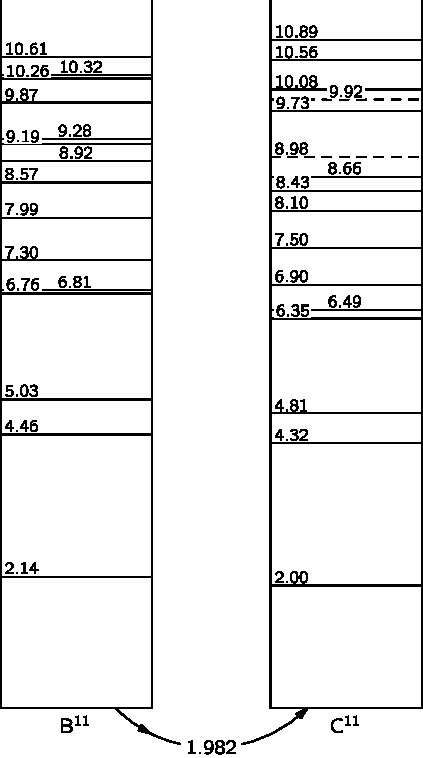
\includegraphics[width=0.8\linewidth]{fyz_fig0184.pdf}
      \caption{Energetické hladiny jader \ce{^{11}B} a \ce{^{11}C} (hodnty udané v
              \si{\protect\mega\protect\electronvolt}). Základní stav \ce{^{11}C} leží o
              \protect\SI{1.982}{\protect\mega\protect\electronvolt} výše než základní stav \ce{^{11}B}
              (\cite[s.~149]{Feynman02}).}
      \label{fyz:fig0184}
    \end{figure}

    Nahradíme-li jeden z neutronů v \ce{^11B} protonem, dostaneme jádro izotopu uhlíku \ce{^11C}.
    Energie nejnižších šestnácti excitovaných stavů \ce{^11C} jsou také naměřeny. Ukazuje je pravá
    polovina obr. \ref{fyz:fig0184}. (Přerušované úsečky vyznačují hladiny, o nichž jsou
    experimentální údaje nedostatečné.)

    Podíváme-li se na obr. \ref{fyz:fig0184}, uvidíme podobnost rozložení hladin energie v obou
    jádrech. První excitované stavy jsou asi \SI{2}{\mega\electronvolt} nad základními stavy.
    Následuje velká mezera asi \SI{2.3}{\mega\electronvolt} k druhému excitovanému stavu, potom malý
    skok pouze \SI{0.5}{\mega\electronvolt} k třetí hladině. Mezi čtvrtou a pátou hladinou je opět
    velký skok, ale mezi pátou a šestou pouze maličká mezera řádu\SI{0.1}{\mega\electronvolt} atd.
    Asi po desáté hladině se zdá, že se shoda ztratila. Je však možné ji postřehnout, označí-li se
    hladiny jejich jinými definičními charakteristikami, například jejich momenty hybnosti a tím,
    jak ztrácejí svou přebytečnou energii.

    Zarážející podobnost v rozložení hladin energie \ce{^11B} a \ce{^11C} zajisté není důsledkem
    náhody. Musí odhalovat nějaký fyzikální zákon. Svědčí vlastně o tom, že i v komplikované situaci
    v jádře způsobí nahrazení neutronu protonem jen velmi malou změnu. Může to znamenat jedině, že
    neutron-neutronové a proton-protonové síly musí být téměř totožné. Pouze tehdy bychom mohli
    očekávat, že jaderná konfigurace se šesti protony a pěti neutrony bude stejná jako konfigurace
    se šesti protony a pěti neutrony.

    Všimněme si, že vlastnosti těchto dvou jader nám neřeknou nic o neutron-protonové síle; v obou
    jádrech je stejný počet neutron-protonových kombinací. Porovnáme-li dvě jádra, taková jako
    \ce{^14C}, které má šest protonů a osm neutronů, a \ce{^14B}, které má jedněch i druhých po
    sedmi, najdeme podobnou shodu hladin energie. Můžeme proto udělat závěr, že p-p, n-n a p-n síly
    jsou identické v celé jejich spletitosti. V zákonech jaderných sil se uplatňuje neočekávaný
    princip. I když síla působící mezi každým párem jaderných částic je velmi komplikovaná, síla
    mezi třemi odlišnými páry je stejná.

    Ale nějaké rozdíly přece jen existují. Hladiny energie nesouhlasí přesně; kromě toho základní
    stav \ce{^11C} má absolutní energii (hmotnost) větší než základní stav \ce{^11B} o
    \SI{1.982}{\mega\electronvolt}. Všechny ostatní hladiny mají absolutní energii také větší o tuto
    hodnotu. Síly tedy nejsou přesně stejné. Velmi dobře však víme, že výsledné síly nejsou přesně
    totožné; mezi dvěma protony působí elektrická síla, neboť každý z nich má kladný elektrický
    náboj, zatímco mezi dvěma neutrony taková síla není. Můžeme snad rozdíly mezi \ce{^11B} a
    \ce{^11C} vysvětlit skutečností, že elektrická interakce je v těch to dvou případech odlišná?
    Snad i menší rozdíly přetrvávající v hladinách jsou vyvolány elektrickými účinky? Protože
    jaderné síly mnohonásobně převyšují elektrickou sílu, elektrické efekty mají na energie hladin
    pouze malý rušivý účinek.

    Abychom tuto myšlenku prověřili nebo spíše zjistili, jaké má důsledky, uvažujme nejdříve energie
    základních stavů obou jader. Abychom přitom měli jednoduchý model, předpokládejme, že jádra jsou
    koule s poloměrem \(r\) (jenž je třeba určit) obsahující \(Z\) protonů. Pokládáme-li jádro za
    kouli s homogenní hustotou náboje, očekáváme, že jeho elektrostatická energie (ze vztahu
    (\ref{fyz:eq874})) bude
    \begin{equation}\label{fyz:eq892}
      W=−\dfrac{3}{5}\dfrac{(Zq_e)^2}{4π\varepsilon_0r},
    \end{equation}
    kde \(q_e\) je elementární náboj protonu. \(Z\) má hodnotu pět pro \ce{^11B} a šest pro
    \ce{^11C}, a tak se jejich elektrostatické energie budou lišit.
    
    Při takovém malém počtu protonů však vztah (\ref{fyz:eq892}) není docela správný. Počítáme-li
    energii mezi všemi páry protonů, přičemž tyto pokládáme za body přibližné rovnoměrně rozdělené v
    objemu koule, zjistíme, že ve vztahu (\ref{fyz:eq892}) je nutné veličinu \(Z^2\) nahradit
    výrazem \(Z(Z - 1)\), takže energii vyjadřuje vztah
    \begin{equation}\label{fyz:eq893}
      W=\dfrac{3}{5}\dfrac{Z(Z−1)q^2_e}{4π\varepsilon_0r}=\dfrac{3}{5}\dfrac{Z(Z−1)}{r}e^2.
    \end{equation}
    Kdybychom znali poloměr jádra \(r\), mohli bychom pomocí (\ref{fyz:eq893}) najít rozdíl
    elektrostatických energií mezi \ce{^11B} a \ce{^11C}. Ale postupujme naopak; namísto toho
    použijme naměřený rozdíl energií k výpočtu poloměru za předpokladu, že celý rozdíl energií má
    elektrostatický původ.

    To však není docela pravda. Rozdíl energií \SI{1.982}{\mega\electronvolt} mezi základními stavy
    \ce{^11B} a \ce{^11C} zahr­nuje klidové energie, tj. energie \(mc^2\), všech částic. Při
    přechodu od \ce{^11B} k \ce{^11C} nahrazujeme neutron protonem, jenž má menší hmotnost. Tak část
    rozdílu energií představuje rozdíl klidových energií neutronu a protonu,
    tj.\SI{0.784}{\mega\electronvolt}. Rozdíl, který je třeba vysvětlit elektrostatickou energií, je
    tak větší než \SI{1.982}{\mega\electronvolt}:
    \begin{equation*}
      \num{1.982} + \num{0.784} = \SI{2.766}{\mega\electronvolt}
    \end{equation*}

    Dosadíme-li tuto hodnotu do (\ref{fyz:eq893}), vypočteme, že poloměr jádra \ce{^11B} nebo
    \ce{^11C} je
    \begin{equation}\label{fyz:eq894}
      r = \SI{3.12e-15}{\m}.
    \end{equation}

    Má takové číslo nějaký smysl? Abychom zjistili, zda ano, musíme jej porovnat s nějakým jiným
    určením poloměru těchto jader. Například jiné měření poloměru jádra můžeme vykonat pozorováním,
    jak jádro rozptyluje rychlé částice. Z takových měření se zjistilo, že hustota látky je ve všech
    jádrech skoro stejná, tj. jejich objemy jsou přímo úměrné počtu částic v nich. Udává-li \(A\)
    počet protonů a neutronů v jádře (číslo, které je přímo úměrné hmotnosti jádra), ukazuje se, že
    jeho poloměr určuje vztah
    \begin{equation}\label{fyz:eq895}
      r=A^{\frac{1}{3}}r_0,
    \end{equation}
    kde
    \begin{equation}\label{fyz:eq896}
      r_0=\SI{1.2e-15}{\m}
    \end{equation}
    Z těchto měření zjistíme, že poloměr jádra \ce{^11B} (nebo \ce{^11C}) by měl být
    \begin{equation*}
      r=11^\frac{1}{3}\cdot\SI{1.2e-15}{\m} = \SI{2.7e-15}{\m}.
    \end{equation*}
    Porovnáme-li tento výsledek s (\ref{fyz:eq894}), vidíme, že naše předpoklady o elektrostatické
    příčině rozdílu energií mezi \ce{^11B} a \ce{^11C} jsou zhruba správné; rozdíl představuje pouze
    asi \SI{15}{\percent} (to není špatné na náš první jaderný výpočet!).

    Příčina rozdílu spočívá pravděpodobně v tomto. Podle současného chápání jader vytváří párový
    počet jaderných částic - v případě \ce{^11B} pět neutronů spolu s pěti protony - jakousi
    uzavřenou vrstvu když se k této vrstvě přidá ještě jedna částice, namísto toho, aby se pohltila,
    zůstane obíhat vně uzavřené vrstvy. Je-li to tak, musíme pro dodatečný proton vzít odlišnou
    elektrostatickou energii. Měli bychom položit přírůstek energie \ce{^11C} vzhledem k \ce{^11B}
    rovný hodnotě výrazu
    \begin{equation*}
      \dfrac{Z_Bq^2_e}{4π\varepsilon_0r}
    \end{equation*}
    tj. energii potřebnou k tomu, aby se na vnější stranu uzavřené vrstvy přidal proton. Tato
    hodnota je právě 5/6 té, kterou předpovídá vzorec (\ref{fyz:eq893}), takže nová předpověď
    poloměru je rovna 5/6 hodnoty vypočtené podle (\ref{fyz:eq894}). Tento výsledek je v mnohem
    těsnější shodě s tím, co se přímo naměřilo.

    Z této shody můžeme udělat dva závěry. První: zdá se, že elektrické zákony platí i v takových
    malých rozměrech jako \SI{10e-15}{\m}. Druhý: přesvědčili jsme se o pozoruhodné shodě
    spočívající v tom, že neelektrické části síly mezi protonem a protonem, neutronem a neutronem a
    protonem a neutronem jsou všechny stejné.
    
  \section{Energie v elektrostatickém poli}\label{fyz:IIchapVIsecV}   
    Zabývejme se nyní jinými metodami výpočtu elektrostatické energie. Všechny se dají odvodit ze
    základního vztahu (\ref{fyz:eq870}), který obsahuje sumu vzájemných energií každého páru nábojů,
    vypočtenou přes všechny páry. Nejdřív chceme napsat výraz pro energii rozdělení nábojů. Jako
    obvykle, předpokládáme, že každý objemový element \(\dd{V}\) obsahuje element náboje
    \(ρ\dd{V}\). Vztah (\ref{fyz:eq870}) je pak třeba zapsat takto:
    \begin{equation}\label{fyz:eq897}
      W=\dfrac{1}{2}\limitint_{\mathclap{\substack{\text{celý}\\\text{prostor}}}}ρ(1)ρ(2)
                    \dfrac{4π\varepsilon_0}{r_{12}}\dd{V_1}\dd{V_2}.
    \end{equation}
    Všimněme si součinitele 1/2, který byl zaveden proto, že ve dvojném integrálu podle \(\dd{V_1}\)
    i \(\dd{V_2}\) jsme všechny páry elementů náboje započítali dvakrát. Neexistuje vhodný způsob,
    jak zapsat integrál, v němž by se každý pár bral v úvahu jen jednou. Dále si všimněme, že
    integrál přes \(\dd{V_2}\) v (\ref{fyz:eq897}) vyjadřuje právě potenciál v bodě \((1)\). Tedy
    \begin{equation*}
      \int\dfrac{ρ(2)}{4π\varepsilon_0r_{12}}\dd{V_2}=ϕ(1),
    \end{equation*}
    takže vztah můžeme psát takto
    \begin{equation*}
      W=\dfrac{1}{2}\intρ(1)ϕ(1)\d{V_1}.
    \end{equation*}
    Protože bod \((2)\) už zde nefiguruje, můžeme prostě psát
    \begin{equation}\label{fyz:eq898}
      W=\dfrac{1}{2}\intρϕ\dd{V}.
    \end{equation}
    Tento vztah lze interpretovat takto. Potenciální energie náboje \(ρ\dd{V}\) je dána součinem
    tohoto náboje a potenciálu v témže bodě. Celková energie je proto rovna integrálu \(ϕρ\dd{V}\).
    Ale opět je tu součinitel \(1/2\). Je ještě potřebný, neboť energie přitom počítáme dvakrát.
    Vzájemná energie dvou nábojů je rovna součinu jednoho z nich a potenciálu v jeho poloze
    vyvolaného druhým nábojem. Nebo je možné ji dostat jako součin druhého náboje a potenciálu v
    jeho poloze vyvolaného prvním nábojem. Pro dva bodové náboje bychom tedy psali
    \begin{align}
      W&=q_1ϕ(1)=q_1\dfrac{q_2}{4π\varepsilon_0r_{12}}  \nonumber \\
      \shortintertext{nebo}
      W&=q_2ϕ(2)=q_2\dfrac{q_1}{4π\varepsilon_0r_{12}}. \nonumber \\
      \shortintertext{Všimněte si, že bychom mohli také napsat, že}
      W&=\dfrac{1}{2}\left[q_1ϕ(1)+q_2ϕ(2)\right].  \label{fyz:eq899}
    \end{align}
    Integrál v (\ref{fyz:eq898}) odpovídá součtu obou členů v závorkách ve vztahu (\ref{fyz:eq899}).
    Proto je potřebný součinitel \(1/2\).

    Zajímavá otázka je: kde sídlí elektrostatická energie? Nebo by bylo možné se ptát: Není to
    jedno? Jaký smysl má tato otázka? Existuje-li pár na sebe působících nábojů, má tato kombinace
    určitou energii. Potřebujeme vůbec mluvit o tom, že tato energie sídlí na jednom nebo na druhém
    z nábojů nebo na obou současně, nebo někde mezi nimi? Tyto otázky snad nemají smysl, protože ve
    skutečnosti pouze víme, že celková energie se zachovává. Představa o tom, že energie někde
    sídlí, není nevyhnutelná.

    A přesto předpokládáme, že opravdu má smysl tak jako v případě tepelné energie i obecně říkat,
    že energie je lokalizována v určitém místě. Pak bychom mohli náš princip zachování energie
    rozšířit o myšlenku, že mění-li se energie v daném objemu, můžeme tuto změnu vysvětlit tokem
    energie do tohoto objemu nebo z něj ven. Chápeme, že naše původní formulace principu zachování
    energie je nadále zcela v pořádku v případě, kdy se nějaká energie ztrácí na jednom místě a
    objevuje se někde jinde velmi daleko aniž by se něco dělo (tj. aniž by nastávaly nějaké zvláštní
    jevy) v prostoru mezi těmito místy. Proto nyní mluvíme o rozšíření principu zachování energie.
    Nazveme to principem \emph{lokálního zachování energie}. Podle tohoto principu se v jakémkoliv
    daném objemu energie mění pouze o to množství, které do tohoto objemu vtéká nebo z něj vytéká.
    Je skutečně možné, že energie se zachovává takovýmto způsobem lokálně. Pokud ano, měli bychom k
    dispozici mnohem detailnější zákon než prostý výrok o zachování celkové energie. Ukazuje se, že
    v přírodě je \emph{energie zachovávána lokálně}. Můžeme najít vzorce, jež udávají, kde je
    energie lokalizována a jak přechází z místa na místo.

    Existuje i \emph{fyzikální} důvod, proč je naléhavé, abychom dokázali určit, kde je energie
    lokalizována. Podle teorie gravitace je každá hmotnost zdrojem gravitační přitažlivosti. Za
    vztahu \(E=mc^2\) také víme, že hmotnost a energie jsou ekvivalentní. Všechna energie je proto
    zdrojem gravitační síly. Pokud bychom nemohli lokalizovat energii, nemohli bychom lokalizovat
    žádnou hmotnost. Nebyli bychom schopni ani určit, kde se nachází zdroje gravitačního pole.
    Teorie gravitace by byla neúplná.

    Když se omezíme na elektrostatiku, skutečně neexistuje způsob, jak se dovědět, kde se energie
    nachází. Úplné Maxwellovy rovnice elektrodynamiky nám však poskytují mnohem víc informací
    (ačkoliv ani potom odpověď není, přesně řečeno, jednoznačná). Tuto otázku budeme proto opět
    podrobněji rozebírat později. Nyní zde uvedeme pouze výsledek pro zvláštní případ - pro
    elektrostatiku. Energie je soustředěna v prostoru, kde se nachází elektrické pole. Vypadá to
    rozumně, neboť víme, že jsou-li náboje urychlovány, vyzařují elektrická pole. Rádi bychom řekli,
    že přecházejí-li světlo nebo rádiové vlny z jednoho bodu do druhého, nesou s sebou energii
    těchto nábojů. Ale ve vlnách nejsou žádné náboje. Proto bychom rádi energii lokalizovali tam,
    kde je elektromagnetické pole, a ne v nábojích, ze kterých pole vzniklo. Takovým způsobem
    popisujeme energii nikoliv pomocí nábojů, ale pomocí polí vytvářených náboji. Můžeme opravdu
    ukázat, že vztah (\ref{fyz:eq898}) je číselně roven hodnotě
    \begin{equation}\label{fyz:eq900}
      W=\dfrac{\varepsilon_0}{2}\int\vec{E}\cdot\vec{E}\dd{V}.
    \end{equation}
    Tento vzorec si můžete vysvětlovat tak, že podle něj v prostoru, kde existuje elektrické pole je
    soustředěna energie, jejíž hustotu (energii připadající na jednotku objemu) vyjadřuje vztah
    \begin{equation}\label{fyz:eq901}
      w=\dfrac{\varepsilon_0}{2}\vec{E}\cdot\vec{E}=\dfrac{\varepsilon_0E^2}{2}.
    \end{equation}
    Tuto představu ilustruje obr. \ref{fyz:fig0185}

    \begin{figure}[ht!]  %\ref{fyz:fig0185}
      \centering
      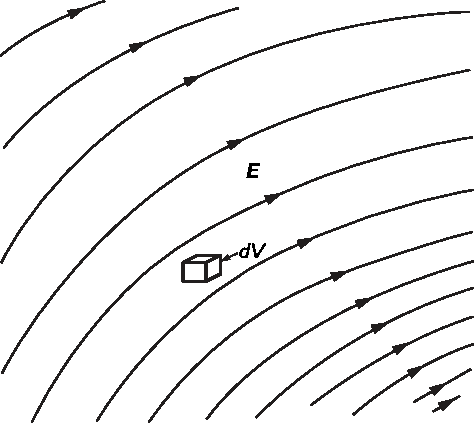
\includegraphics[width=0.6\linewidth]{fyz_fig0185.pdf}
      \caption{Každý element objemu \(\dd{V} = \dd{x}\dd{y}\dd{z}\) v elektrickém  poli obsahuje
      energii \(\varepsilon_0/2E^2\dd{V}\) (\cite[s.~154]{Feynman02}).}
      \label{fyz:fig0185}
    \end{figure}

    Abychom ukázali, že vztah (\ref{fyz:eq900}) vyhovuje našim zákonům, začneme dosazením vztahu
    mezi \(ρ\) a \(ϕ\) tedy
    \begin{equation*}
      ρ=−\varepsilon_0∇^2ϕ.
    \end{equation*}
    který jsme dostali v kapitole \ref{fyz:IIchapV}, do výrazu na pravé straně (\ref{fyz:eq898}).
    Tím dostaneme
    \begin{equation}\label{fyz:eq902}
      W=−\dfrac{\varepsilon_0}{2}∫ϕ∇^2ϕ\dd{V}.
    \end{equation}
    Rozepíšeme-li integrand do složek, uvidíme, že
    \begin{gather*}
      \begin{align*}
        ϕ∇^2ϕ &=ϕ\left(\diffp[2]{ϕ}{x}+\diffp[2]{ϕ}{y}+\diffp[2]{ϕ}{z}\right)      \\
              &=\diffp{}{x}\left(ϕ\diffp{ϕ}{x}\right)−\left(\diffp{ϕ}{x}\right)^2  \\
              &+\diffp{}{y}\left(ϕ\diffp{ϕ}{y}\right)−\left(\diffp{ϕ}{y}\right)^2  \\
              &+\diffp{}{z}\left(ϕ\diffp{ϕ}{z}\right)−\left(\diffp{ϕ}{z}\right)^2  \\
              &=∇⋅(ϕ∇ϕ)−(∇ϕ)⋅(∇ϕ).
      \end{align*}
    \end{gather*}
    Náš intergrál je potom
    \begin{equation*}
      W = \dfrac{\varepsilon_0}{2}\int(∇ϕ)⋅(∇ϕ)\dd{V}−\dfrac{\varepsilon_0}{2}\int∇⋅(ϕ∇ϕ)\dd{V}.
    \end{equation*}
    Pomocí Gaussovy věty můžeme druhý integrál transformovat na plošný integrál
    \begin{equation}\label{fyz:eq903}
      \int\limits_{\mathclap{objem}}∇⋅(ϕ∇ϕ)\dd{V} = 
      \int\limits_{\mathclap{povrch}}(ϕ∇ϕ)\cdot\vec{n}\dd{S}.
    \end{equation}

    Tento plošný integrál vypočteme pro případ, že plocha sahá do nekonečna (takže objemové
    integrály se stanou integrály přes celý prostor), a za předpokladu, že všechny náboje jsou
    umístěny v nějaké konečné vzdálenosti. Jednoduchý způsob, jak postupovat, je vzít kulovou plochu
    s velmi velkým poloměrem \(R\), jejíž střed se nachází v počátku souřadnicové soustavy. Víme, že
    když jsme velmi daleko od všech nábojů, mění se \(ϕ\) jako \(1/R\) a \(∇ϕ\) jako \(1/R^2\). (Obě
    veličiny budou klesat s \(R\) ještě rychleji, když sumární náboj rozdělení je roven nule.)
    Protože plošný obsah povrchu velké koule roste jako \(R^2\), vidíme, že při zvětšování poloměru
    koule klesá plošný integrál jako \((1/R) (1/R^2)R^2 = 1/R\). Zahrneme-li tedy do našeho
    integrování celý prostor \((R\rightarrow\infty)\), plošný integrál se bude blížit k nule a
    dostaneme
    \begin{equation}\label{fyz:eq904}
      W=\dfrac{\varepsilon_0}{2} \int\limits_{\mathclap{\text{celý prostor}}}(∇ϕ)(∇ϕ)\dd{V} = 
        \dfrac{\varepsilon_0}{2} \int\limits_{\mathclap{povrch}}\vec{E}\cdot\vec{E}\dd{V}.
    \end{equation}
    Vidíme, že energii jakéhokoliv rozdělení nábojů můžeme vyjádřit jako integrál hustoty energie 
    sídlící v poli.

  \section{Energie bodového náboje}\label{fyz:IIchapVIsecVI}
    Podle našeho vztahu (\ref{fyz:eq904}) bude i jednotlivý bodový náboj \(q\) mít nějakou
    elektrostatickou energii. V tomto případě vyjádříme intenzitu elektrického pole takto:
    \begin{equation*}
      E=\dfrac{q}{4π\varepsilon_0r^2}.
    \end{equation*}
    Hustota energie ve vzdálenosti \(r\) od náboje je tedy
    \begin{equation*}
      \dfrac{\varepsilon_0E^2}{2}=\dfrac{q^2}{32π^2\varepsilon_0r^4}.
    \end{equation*}
    Jako element objemu můžeme vzít kulovou slupku s tloušťkou \(\dd{r}\) plošným obsahem \(4πr^2\).
    Celková energie je
    \begin{equation}\label{fyz:eq905}
      W =\int_{r=0}^∞\dfrac{q^2}{8π\varepsilon_0r^2}\dd{r}
        =−\left.\dfrac{q^2}{8π\varepsilon_0}\right\rvert^{r=∞}_{r=0}.
    \end{equation}
    Horní hranice \(r=∞\) nepředstavuje žádnou obtíž. V případě bodového náboje bychom však měli
    integrovat až do \(r = 0\), což vede k nekonečně velké hodnotě. Podle vztahu (\ref{fyz:eq904})
    je v poli bodového náboje nekonečné množství energie, ačkoli jsme vyšli z představy, že energie
    existuje pouze mezi bodovými náboji. Do našeho původního vzorce (\ref{fyz:eq870}) pro energii
    soustavy bodových nábojů jsme nezahrnuli žádnou interakční energii náboje se sebou samým. Co se
    potom stalo? Když jsme přešli ke spojitému rozdělení náboje ve vztahu (\ref{fyz:eq897}),
    započítali jsme energii interakce každého infinitezimálního náboje se všemi ostatními
    infinitezimálními náboji. Stejný zápočet byl proveden ve vztahu (\ref{fyz:eq904}), takže když
    používáme (\ref{fyz:eq904}) pro konečný bodový náboj, zahrnujeme i energii, která je
    spotřebována na to, aby se daný náboj sestavil z infinitezimálních částí. Skutečně si všimněme,
    že kdybychom pro energii nabité koule použili náš výraz (\ref{fyz:eq878}) a nechali poloměr
    blížit se nule, také bychom dostali výsledek (\ref{fyz:eq905})

    Musíme udělat závěr, že představa o tom, že energie sídlí v poli, se neshoduje s předpokladem o
    existenci bodového náboje. Jedním východiskem z tohoto problému je prohlásit, že elementární
    částice, takové jako elektron, nejsou body, ale ve skutečnosti malými rozděleními náboje. Mohli
    bychom však také říct, že něco chybného je v naší teorii elektřiny při velmi malých
    vzdálenostech anebo v představě o lokálním zachování energie. S každým z těchto hledisek jsou
    problémy. Tyto problémy nebyly nikdy překonány a existují dodnes. Někdy později, až budeme
    mluvit o některých dalších pojmech jako např. hybnost v elektromagnetickém poli, podáme úplnější
    výklad těchto fundamentálních problémů v našem chápání přírody.